% Diese Zeile bitte -nicht- aendern.
\documentclass[course=asp]{aspdoc}

%newly added packages
\usepackage{microtype}
\usepackage{graphicx}
\usepackage{wrapfig}
\usepackage{enumitem}
\usepackage{amssymb}

\usepackage{amsmath}	%eins von beidem?
\usepackage{mathtools}

\usepackage{index}

%%%%%%%%%%%%%%%%%%%%%%%%%%%%%%%%%
%% TODO: Ersetzen Sie in den folgenden Zeilen die entsprechenden -Texte-
%% mit den richtigen Werten.
\newcommand{\theGroup}{132} % Beispiel: 42
\newcommand{\theNumber}{A214} % Beispiel: A123
\author{Mohammed Attia \and Patrick Zimmermann \and Thomas Torggler}
\date{Wintersemester 2020/21} % Beispiel: Wintersemester 2019/20
%%%%%%%%%%%%%%%%%%%%%%%%%%%%%%%%%

% Diese Zeile bitte -nicht- aendern.
\title{Gruppe \theGroup{} -- Abgabe zu Aufgabe \theNumber}

\begin{document}
\maketitle

\newpage
\section{Einleitung}

Raumfüllende Kurven bilden die Brücke zwischen Kunst und mathematischer Geometrie. In der Mathematik werden sie gemeinhin benutzt um ein n-dimensionales Problem in ein eindimensionales zu konvertieren. Eine solche Kurve beschreibt essentiell einen linearen Pfad durch n-dimensionale Räume. Giuseppe Peano war der Erste, der eine solche Kurve 1890 definierte.
Um einen n-dimensionalen Raum in die Dimension n-1 zu konvertieren, lässt sich eine stetig surrjektive Funktion $f(x)$ erstellen, so das gilt: $\forall x \in \mathbb{R}^{n-1} \quad \exits y \in \mathbb{R}^n$. Für einen Beweis siehe (Quelle?). Hier wollen wir uns auf die sogenannten Peano-Kurven beschränken. Für eine solche Kurve definieren wir ein Intervall I = [0,1], sowie  $f: I \rightarrow I^2 $. Dann ist die Peano-Kurve: $\lim\limits_{x \to \infty}f(x)$, mit $x \in I$. Sie { entspricht dem Grenzwert einer Folge von Funktionen f(x) und } lässt sich mit der Bedingung, dass sich die Kurve nicht überschneiden darf, folgendermaßen konstruieren:

Man unterteile eine Fläche in 9 Quadrate. Jedes dieser Quadrate soll nun durch eine Kurve besucht werden. Dadurch durchläuft die Kurve die Quadrate in Form eines „S“.
In einem Iterationsschritt lässt sich eines der 9 Quadrate in weitere 9 Quadrate Unterteilen, die wiederum auf selbe Art verbunden werden, wie in Abb.1 gezeigt.

\begin{figure} [ht] %vorher, eigentlich bild unter text
\centering
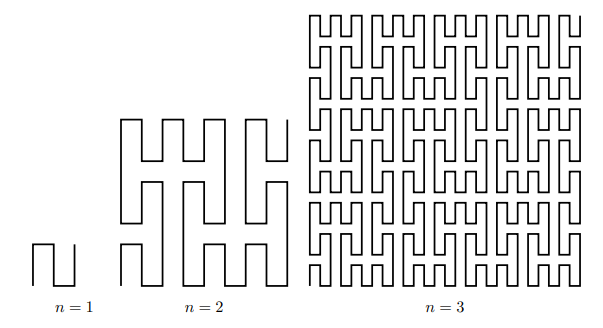
\includegraphics{PeanoBsp.png}
\caption{Peano-Kurve mit n = \{1,2,3\}, ~\cite{aufgabenstellung}}\label{Abb:Peano}		%TEST
\end{figure}

%bilder von n=1 bis n=3, wahrscheinlich seite voll?
Im Folgenden Definieren wir $n \in \mathbb{N}$ als Grad der Kurve.
Wir beschreiben nun unseren Ansatz einen iterativen Algorithmus zu finden, um die eben beschriebene Peano-Kurve darzustellen. %Ergebnis hier einfügen!!

\newpage

\section{Lösungsansatz}
Der Aufbau der Peano-Kurve ermöglicht es die Kurve des aktuellen Grades mit einer Variation der gespiegelten und originalen Kurve des vorherigen Grades zu zeichnen.
Diese Observation war der Grundstein unseres iterativen Algorithmus. Anfangs wird dabei die Startkurve hardcodiert in einem Integer Array abgespeichert wobei die Zahlen von 0 bis 3 jeweils einer der vier Richtungen entsprechen. Falls der eingegebene Grad $n > 1$ ist, wird aufsteigend über alle Grade bis inklusive n iteriert wobei während jedem Schritt die Kurve des vorherigen Grades in der originalen Reihenfolge des ersten Grades entweder im Originalzustand oder gespiegelt acht mal in den Array eingefügt wird, sodass die vollständige Kurve des aktuellen Grades entsteht. 

\begin{figure} 	%ZU GROSS!!
\centering
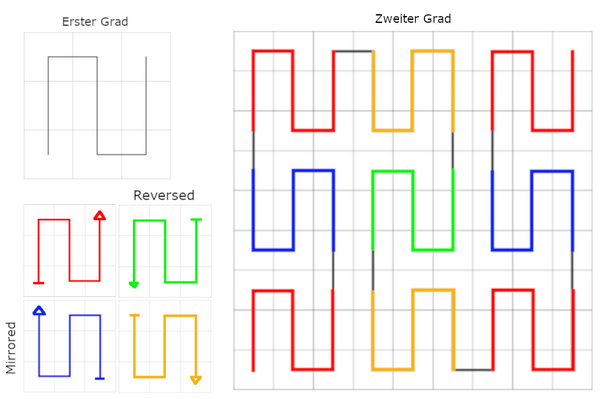
\includegraphics[scale=0.7]{PeanoFarbcodiert.png}
\caption{Peano-Kurve mit n = 1, n = 2}\label{Abb:Peano Lösungsidee}
\end{figure}

Zu beachten ist dabei jedoch, dass durch das Spiegeln und Einfügen von Kurven deren Richtung noch inkorrekt sein könnte, dafür gibt es aber ähnlich zur Spiegelungsmethode eine Methode zum Umkehren der Richtung. Nach diesen Schritten sind die neun erstellten Kurven jedoch noch nicht miteinander verbunden. Da sich das Muster der ursprünglichen Kurve durch alle Grade wiederholt, kann nach jedem Schritt ein hardcodierter Pfad zur nächsten Kurve eingefügt werden.
Nachdem über alle Grade iteriert wurde, läuft der Algorithmus den vollständigen Richtung Array durch, verändert dabei bei jedem Schritt je nach Richtungsangabe entweder die x oder y-Koordinate und speichert diese dann in die Ausgabeliste der Peano-Methode.

\newpage

% TODO: Je nach Aufgabenstellung einen der Begriffe wählen
\section{Korrektheit} % oder Genauigkeit 

%Kurve definieren!

Die Genauigkeit unseres Algorithmus ist abhängig von dem Grad $n$, dass die Anzahl an Iterationen bestimmt, wie in den Abb.1 beschrieben. Das geht auch aus der beschriebenen mathematischen Definition hervor, da die Peano-Kurve an sich ein Grenzwert ist. Somit wird der Algorithmus genauer, je größer der Grad der Kurve ist, da die Punkte auf der Kurve sich ebenfalls einem Grenzwert annähern. Ansonsten ist die Kurve wie ebenfalls schon oben beschrieben definiert, weshalb nur die Korrektheit unseres Algorithmus entscheidend ist.
Grundsätzlich lässt sich die Korrektheit einer Kurve, besonders bei der von uns behandelten, nachweisen indem man ihre graphischen Darstellungen vergleicht. Da das Theoretisch aber nicht möglich ist, folgt auch eine Implementierung in Assambler und C, die wir auch hinsichtlich ihrer Performanz analysieren wollen.
Wir wollen dennoch unseren Ansatz auf Korrektheit prüfen.

Nachdem die Kurve immer wieder die gleichen (elementaren) Bestandteile verwendet, müssen diese und deren Permutationen richtig berechnet werden. Im speziellen sind das die Kurven mit $n = 1$ und $n = 2$. So lässt sich induktiv die Korrektheit beweisen, da wir, wie im vorherigen Kapitel beschrieben, zum berechnen eine Kurve n-ten Grades nur die Kurve selbst sowie die gespiegelte und invertierte Versionen der Kurve vom Grad n-1 benutzen. Bei der "invertierten" Version handelt es sich in diesem Kontext um eine Punktspiegelung im Mittelpunkt der vorhergehenden Kurve, weitere Erläuterungen folgen.

%induktionsbasis
Beginnen wir mit $n = 1$. Hier ist die Kurve vordefiniert, dementsprechend gibt es nichts zu zeigen. Da auf diesem Muster alle anderen Kurven mit $n>1$ basieren, ist sie in unserem Algorithmus ebenfalls als Basis fest gegeben.
Des Weiteren ist die Definition der Kurve mit $n = 2$ für die Berechnung aller weiteren Kurven von Nöten, da man anhand dieser Kurve die Bedingungen der weiteren Konstruktion ableiten kann.
%induktionsannahme
Da die Funktion wie definiert surrjektiv ist, gilt: 

$\forall n>1 \in \mathbb{N}$, $\exists y \in \mathbb{R}^n$ mit $x \in [0,1]$: $f(x)= y$	%evtl ändern...

Dadurch lassen sich Kurven mit höherem Grad konstruieren. Sei nun $n>1$ und beliebig gewählt.
%induktionschritt - evtl Unterkapitel

Betrachten wir nun Kurven mit $n>=2$. Hierzu müssen wir die Permutationen der vorhergehenden Kurve untersuchen, die wir zur Konstruktion der Kurve mit Grad n benötigen.	%Spiegelung
Die gespiegelte Permutation ist im Kern nichts anderes als die normale Peano-Kurve mit anderer Reihenfolge der Koordinatenberechnung, also von $p_1=(1,1)$ nach $p_2 = (0,0)$. Dies hat zur Folge, dass sich außer der Reihenfolge der Punkte an der grundlegenden Kurve nichts ändert. Somit ist die Spiegelung induktiv eben so korrekt wie die zugrundeliegende Kurve niedrigeren Grades.

%Invertierung
Bei der Invertierung wird die Kurve ähnlich zur Achsenspiegelung ebenfalls die vertikale Richtung geändert, jedoch wird weiterhin auch die horizontale Richtung geändert. Die Kurve wird in dem mittlerem Punkt der Kurve gespiegelt. Da die Kurve immer $9^n$ Felder besitzt, existiert immer ein solcher Mittelpunkt. Dadurch wird die vorausgehende Kurve notwendiger weise verändert.  Diese zusätzliche Operation ist ebenfalls elementare Spiegelungen sind und somit direkt auf die Koordinatenberechnung Einfluss haben ohne die Kurve anders zu verändern, ändert sich der charakteristische Verlauf der Kurve nicht.

%Punktsymetrie
Die Eigenschaft der Punktsymetrie lässt sich wie folgt belegen: 
%Verbinden der Permutationen

Die unterschiedlichen Permutationen der Peano-Kurve werden durch eine eben solche Kurve mit $n = 1$ verbunden. Dadurch bleiben alle Eigenschaften der Kurve erhalten, da wir keine weiteren Punkte in die Kurve einfügen. Zudem ist dies teil auch ebenso teil der Definition dieser Kurve. 

%Mathematischen sachen be/ver-weisen!
%Mappen wir in [0,1]? sonst evtl Text ändern!
%Punktsymetrie beweisen!
%verbinden der Kurven!

\newpage
\section{Performanzanalyse}

%Technische Limitationen in C
Bei dem testen unseres Programms fallen bei Graden von $n > 6$ bestimmte technische Limitationen unser Rechensysteme auf. 

Zum einen haben wir kein Programm gefunden, dass die generierten .svg Dateien von einer Größe 43.0 Megabyte (Peano-Kurve mit $n = 7$) öffnen kann. Mit zunehmendem Grad enthält die .svg Dateien immer mehr Punkte der Kurve, weshalb sie ebenfalls exponentiell zur Basis 9 steigt. Deshalb möchten wir an dieser Stelle auf das Kapitel "Korrektheit" verweisen um die Kurve auf selbige zu prüfen.

Zum anderen ist es nicht möglich, beliebig viel Speicher zu allokieren, da die von uns benutzte  "malloc"-Funktion maximal 17.179.869.184 Bytes auf dem Heap allokieren kann und der Heap zusätzlich in seiner Größe begrenzt ist. Deshalb können wir auf unseren Systemen die Funktion mit maximal $n = 9$ ausführen, da sonst nicht genügend Speicher allokiert wird. Für $n = 10$ müssten 27.894.275.208 Bytes allokieren, wozu wir eben nicht im Stande sind, weshalb wir den Wertebereich von $n$ auf $[1;9]$ limitiert haben.

Um zu ermitteln, wie viel Speicher wir allokieren können, haben wir eine For-Schleife  folgenden Typs ausgeführt:

\begin{PseudoCode}	%Formatieren! 
u\_int64\_t *v;    	


for (u\_int64\_t i = 1; v = (u\_int64\_t *) malloc(i); i <<= 1)   

  
\{     

    
print(i);  
	
	      
free(v);    
	
	 
\}
\end{PseudoCode}

%Assembler 


\newpage
\section{Zusammenfassung und Ausblick}

% TODO: Fuegen Sie Ihre Quellen der Datei Ausarbeitung.bib hinzu			!!!!
% Referenzieren Sie diese dann mit \cite{}.									
% Beispiel: CR2 ist ein Register der x86-Architektur~\cite{intel2017man}.
\bibliographystyle{plain}
\bibliography{Ausarbeitung}{}

\end{document}
